\begin{frame}
\frametitle{The Discrete Resonance Spectrogram (DRS)}
	\begin{block}{Overview}
		\begin{itemize}
			\item High resolution spectral analysis of audio signals
			\item Gives precise shape and location of spectral peaks 
			\item Provides access to the content of audio signals
		\end{itemize}
	\end{block}
	\centering
	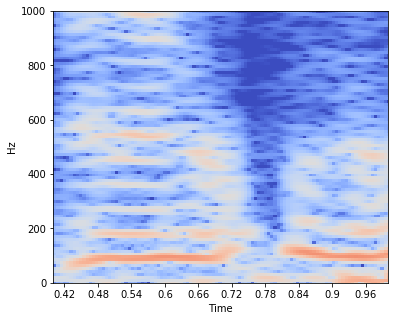
\includegraphics[width=0.45\textwidth]{images/voice-ffts.png}	
	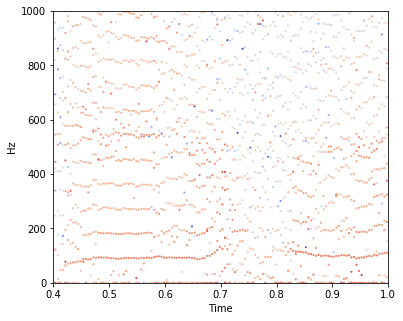
\includegraphics[width=0.45\textwidth]{images/voice-drs.png}	
\end{frame}

\begin{frame}
\frametitle{DRS Advantages and Applications}
	\begin{block}{Target Applications}
		\begin{itemize}
			\item Analysis of voice signals in industrial environments
			\item Vocal signature modelling
			\item Data compression
		\end{itemize}	
	\end{block}
	\begin{block}{Advantages of the DRS}
		\begin{itemize}
			\item Better resolution than FFT based methods
			\item Affords intelligent top-down signal processing
			\item Better integration with symbolic knowledge representation
		\end{itemize}
	\end{block}
\end{frame}

\begin{frame}
\frametitle{Current Objectives}
	\begin{block}{Intelligent bottom-up pattern detection}
		\begin{itemize}
			\item Parameter selection $\checkmark$
			\item Improve time resolution $\checkmark$
			\item Fundamental frequency (F0) tracking $\checkmark$
			\item Source detection and isolation
			\item Noise reduction
		\end{itemize}
	\end{block}
\end{frame}

\begin{frame}
\frametitle{Work to date}
	\begin{columns}
		\begin{column}{0.5\textwidth}
			\begin{block}{Parameter selection \checkmark}	
				An algorithm for automatically selecting parameters, reducing the need for tuning.
			\end{block}
			\begin{block}{Improved time resolution \checkmark}
				A segmentation algorithm which uses smooth sliding window envelopes.
			\end{block}
			\begin{block}{F0 estimation \checkmark}
				An algorithm for tracking fundamental pitch (Geraint).
			\end{block}
		\end{column}
		\begin{column}{0.5\textwidth}
			\begin{tabular}{r l}
				Original signal & $\rhd$ \\
				Basic analysis & $\rhd$  \\ 
				Enhanced analysis & $\rhd$ \\
				& \\
			\end{tabular} 
			\par \scriptsize{F0 tracking works well for simple harmonic sounds such as a flute.} 
			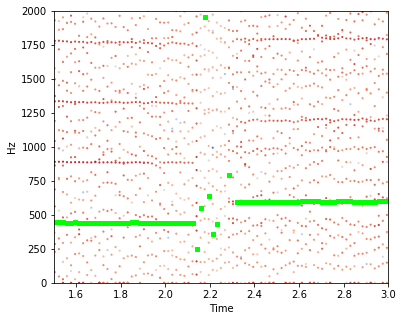
\includegraphics[width=\textwidth]{images/f0-flute.png}
		\end{column}
	\end{columns}			
\end{frame}

\begin{frame}
\frametitle{Immediate Next Steps}
	\begin{columns}
		\begin{column}{0.5\textwidth}
			\begin{block}{Phase and decay}	
				Improve F0 tracking using phase and decay information
			\end{block}
			\begin{block}{Inter-slice information}
				Use previous slice to inform analysis. 
			\end{block}
			\begin{block}{Source isolation}
				Use F0 information to detect and isolate individual sources.
			\end{block}
		\end{column}
		\begin{column}{0.5\textwidth}
			\scriptsize{F0 tracking deteriorates for more complex sounds such as a voice.} 
			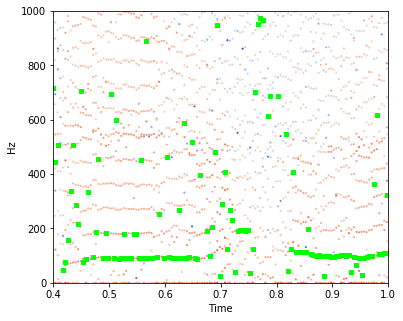
\includegraphics[width=\textwidth]{images/f0-voice.png}
		\end{column}
	\end{columns}			
\end{frame}